\chapter{Software Implementation}
\label{ch:software}
The methodology of Chapter~\ref{ch:method} is implemented as an open Python package, an experiment pipeline, a
tutorial notebook and a graphical application. This chapter describes their structure and use. All components run in a
single environment pinned with the \texttt{uv} package manager (Python 3.12), and all input data are streamed from the
Microsoft Planetary Computer without registration and cached locally \cite{planetary}.

\section{Software Architecture}
The package \texttt{sarsim} contains five modules, each responsible for one stage of the data flow of
Fig.~\ref{fig:dataflow}. The module \texttt{data} provides cached access to the Copernicus GLO-30 DEM, to the window of
a Sentinel-1 GRD product that covers the DEM together with its annotation and calibration files, and to the ESA
WorldCover map. The module \texttt{s1} parses the product annotation, fits the orbit polynomial, solves the
zero-Doppler condition, applies the piece-wise slant-to-ground-range conversion and calibrates digital numbers to
$\sigma^0$. The module \texttt{rdsim} computes the facet geometry block-wise, flags shadow and layover, evaluates the
backscatter laws and renders the simulated image by bilinear splatting. The module \texttt{compare} implements
multilooking, sub-pixel co-registration, the similarity metrics and back-geocoding to the DEM grid. The module
\texttt{geodesy}, finally, provides the conversions between geodetic and Earth-centred coordinates and the EGM2008
geoid undulation. The repository structure is listed in Appendix~\ref{app:structure}.

\section{Experiment Pipeline}
The script \texttt{run\_all.py} carries out experiments E1 to E5 of Section~\ref{sec:final-design} and
Chapter~\ref{ch:method} in one run: it downloads and caches the data, computes the facet geometry once per scene,
renders the five backscatter laws, evaluates both viewing geometries, repeats the simulation for the sensitivity
cases and analyses the residuals per land-cover class. All numbers are written to \texttt{results/metrics.json} and to
CSV tables, and all figures of Chapter~\ref{ch:results} that are prefixed with ``E'' are written to
\texttt{figures/pipeline/}. The tables and numbers quoted in this report are generated from \texttt{metrics.json} by
the script \texttt{report/make\_tables.py}, so that the text cannot drift from the results. A complete run takes about
fifteen minutes on a laptop with 16\,GB of memory.

\section{Verification and Testing}
Eight unit tests guard the geometric core of the simulator. They check that flat terrain produces neither shadow nor
layover, that steep fore-slopes and back-slopes are classified as layover and shadow, that gentle slopes are
classified as neither, that the backscatter laws decrease monotonically, that the bilinear splatting conserves energy,
that the geodetic conversion is exact at the equator and the pole, that the block-wise facet geometry does not depend on
the block size, and that the range-Doppler geocoding reproduces the zero-Doppler times and pixel positions of the
geolocation grid of a real Sentinel-1 product. All tests pass.

\section{Tutorial Notebook}
The notebook \texttt{notebooks/01\_sar\_simulation\_walkthrough.ipynb} reproduces the verification sequence of
Section~\ref{sec:res-verif} step by step: a single point target and pulse, a line of targets, the moving satellite with
raw, range-compressed and focused data, a flat surface with speckle, a sinusoidal surface, a real DEM patch, the
geometric distortions, the radiometric chain and, finally, the comparison with a real Sentinel-1 scene. Each step is
shown as a sequence of plots that follows the processing chain, which makes the notebook usable as teaching material.

\section{Graphical Application}
\label{sec:gui}
To make the simulator usable without programming, a graphical application was developed with the Streamlit framework.
It runs the complete simulation for a DEM of any location and returns the simulated SAR data in formats suitable for
research use. As illustrated in Fig.~\ref{fig:gui-start}, all inputs are grouped in a sidebar and a single
\emph{Run simulation} button starts the processing, while the main area is divided into an \emph{Overview} and a
\emph{Results} tab. An information button in the top-right corner opens a panel that explains how to use the
application and how the simulation works (Fig.~\ref{fig:gui-info}).

The terrain can be selected from presets, defined by a bounding box, in which case the Copernicus GLO-30 DEM is
downloaded and cached, or uploaded as a GeoTIFF in any projection, which is reprojected to geographic coordinates.
Two geometry modes are offered. The generic mode simulates a Sentinel-1-like sensor on a straight orbit at 693\,km over
a flat Earth for any location and works offline once the DEM is available; the user chooses the pass (ascending,
looking east, or descending, looking west), the look angle and, optionally, the heading, the pixel spacing and the
orbit height. The real mode searches the Sentinel-1 catalogue for a scene covering the area, simulates in the exact
geometry of that product with the methodology of Chapter~\ref{ch:method}, and compares the simulation with the real
image using the metrics of Section~\ref{sec:res-verif} and Chapter~\ref{ch:results}. The backscatter law is selected
among the five laws of Table~\ref{tab:models}, with the fitted law as the default, and speckle and multilooking can be
added. A memory guard limits the number of facets by reducing the oversampling and, if necessary, aggregating the DEM,
and reports when it does so.

After a run, the Overview tab summarises the area, the DEM grid, the height range, the fractions of layover and
shadow and the run time, together with a hillshade of the terrain and the configuration used
(Fig.~\ref{fig:gui-overview}). The Results tab shows the simulated $\sigma^0$ in radar and in map geometry, the layover
and shadow masks, the local incidence angle with its histogram and the $\sigma^0$ curve against the local incidence
angle, and, in the real mode, the real and simulated images side by side with a density scatter plot and the
agreement metrics (Fig.~\ref{fig:gui-results}). A download button provides a ZIP archive that contains map-geometry
GeoTIFFs of the simulated $\sigma^0$ (linear and in dB), the local incidence angle, the layover and shadow masks and the
DEM used, the radar-geometry image as GeoTIFF and NumPy array, and a metadata file that records all inputs, sensor
parameters and the software version. The full Innsbruck scene is simulated in about 10\,s in the generic mode and
about 35\,s in the real mode, and the application is covered by headless tests that run the complete pipeline from the
\emph{Run simulation} button.

\begin{figure}[htbp]
\centering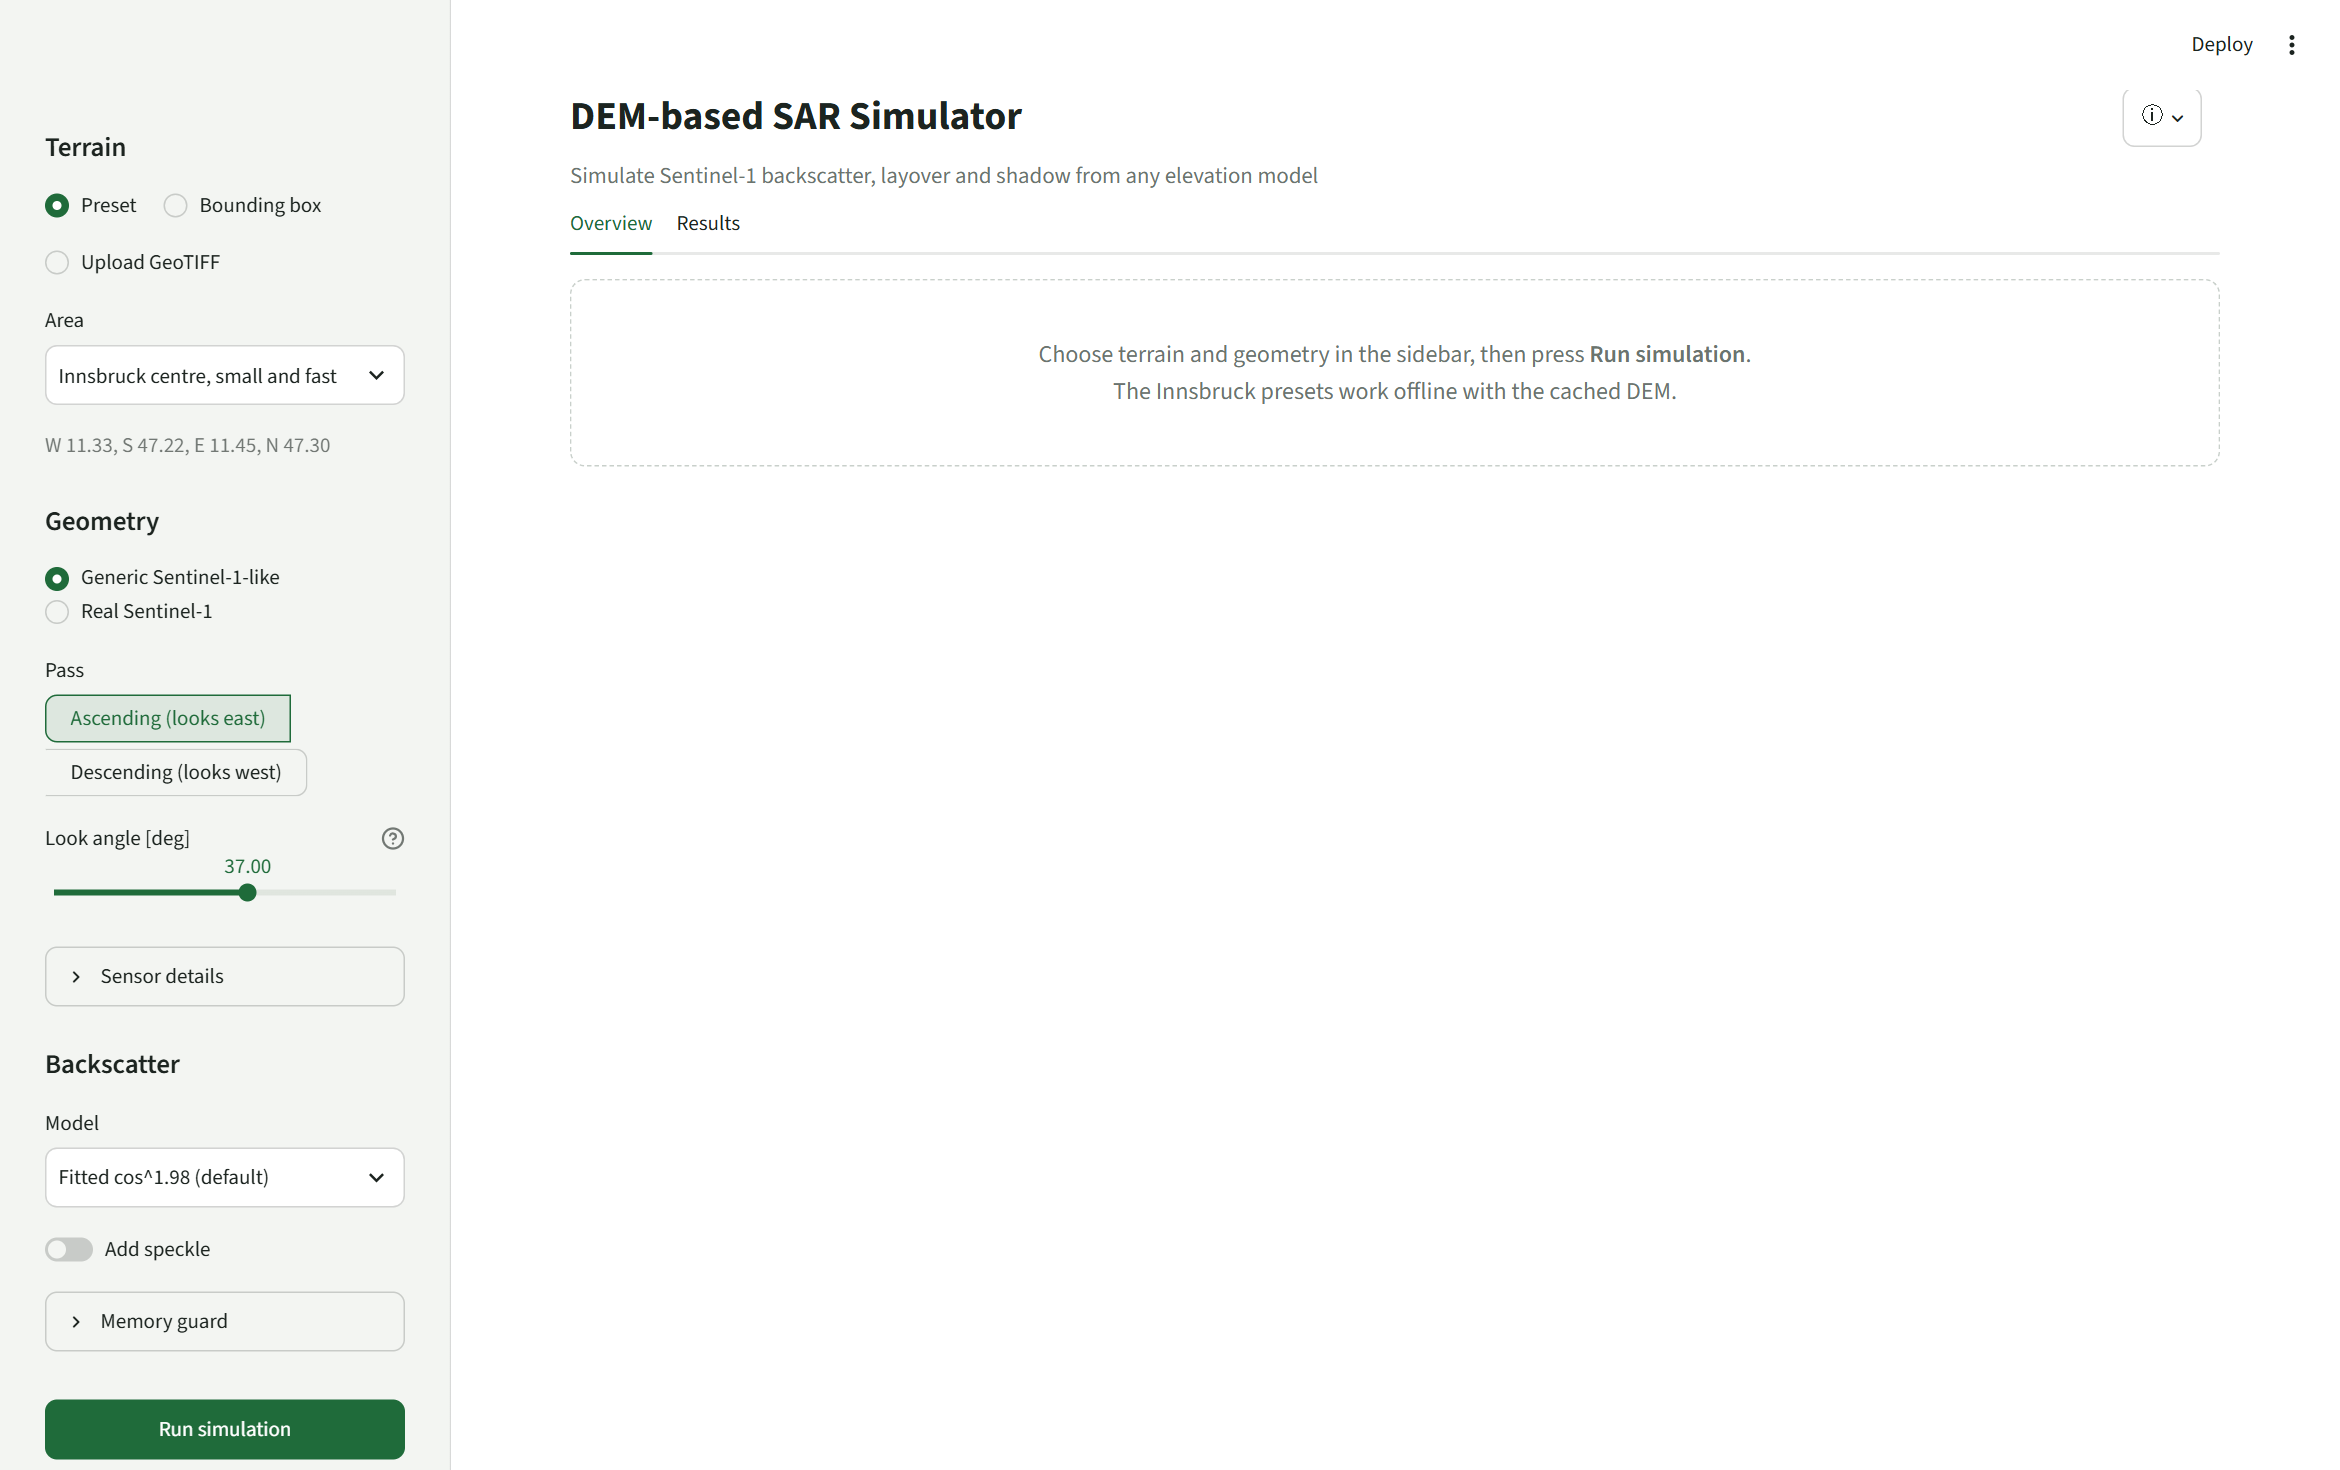
\includegraphics[width=\textwidth]{gui_01_start.png}
\caption[Graphical application: start page]{Graphical application: start page with the input sidebar (terrain,
geometry, backscatter, memory guard) and the information button in the top-right corner.}
\label{fig:gui-start}
\end{figure}
\begin{figure}[htbp]
\centering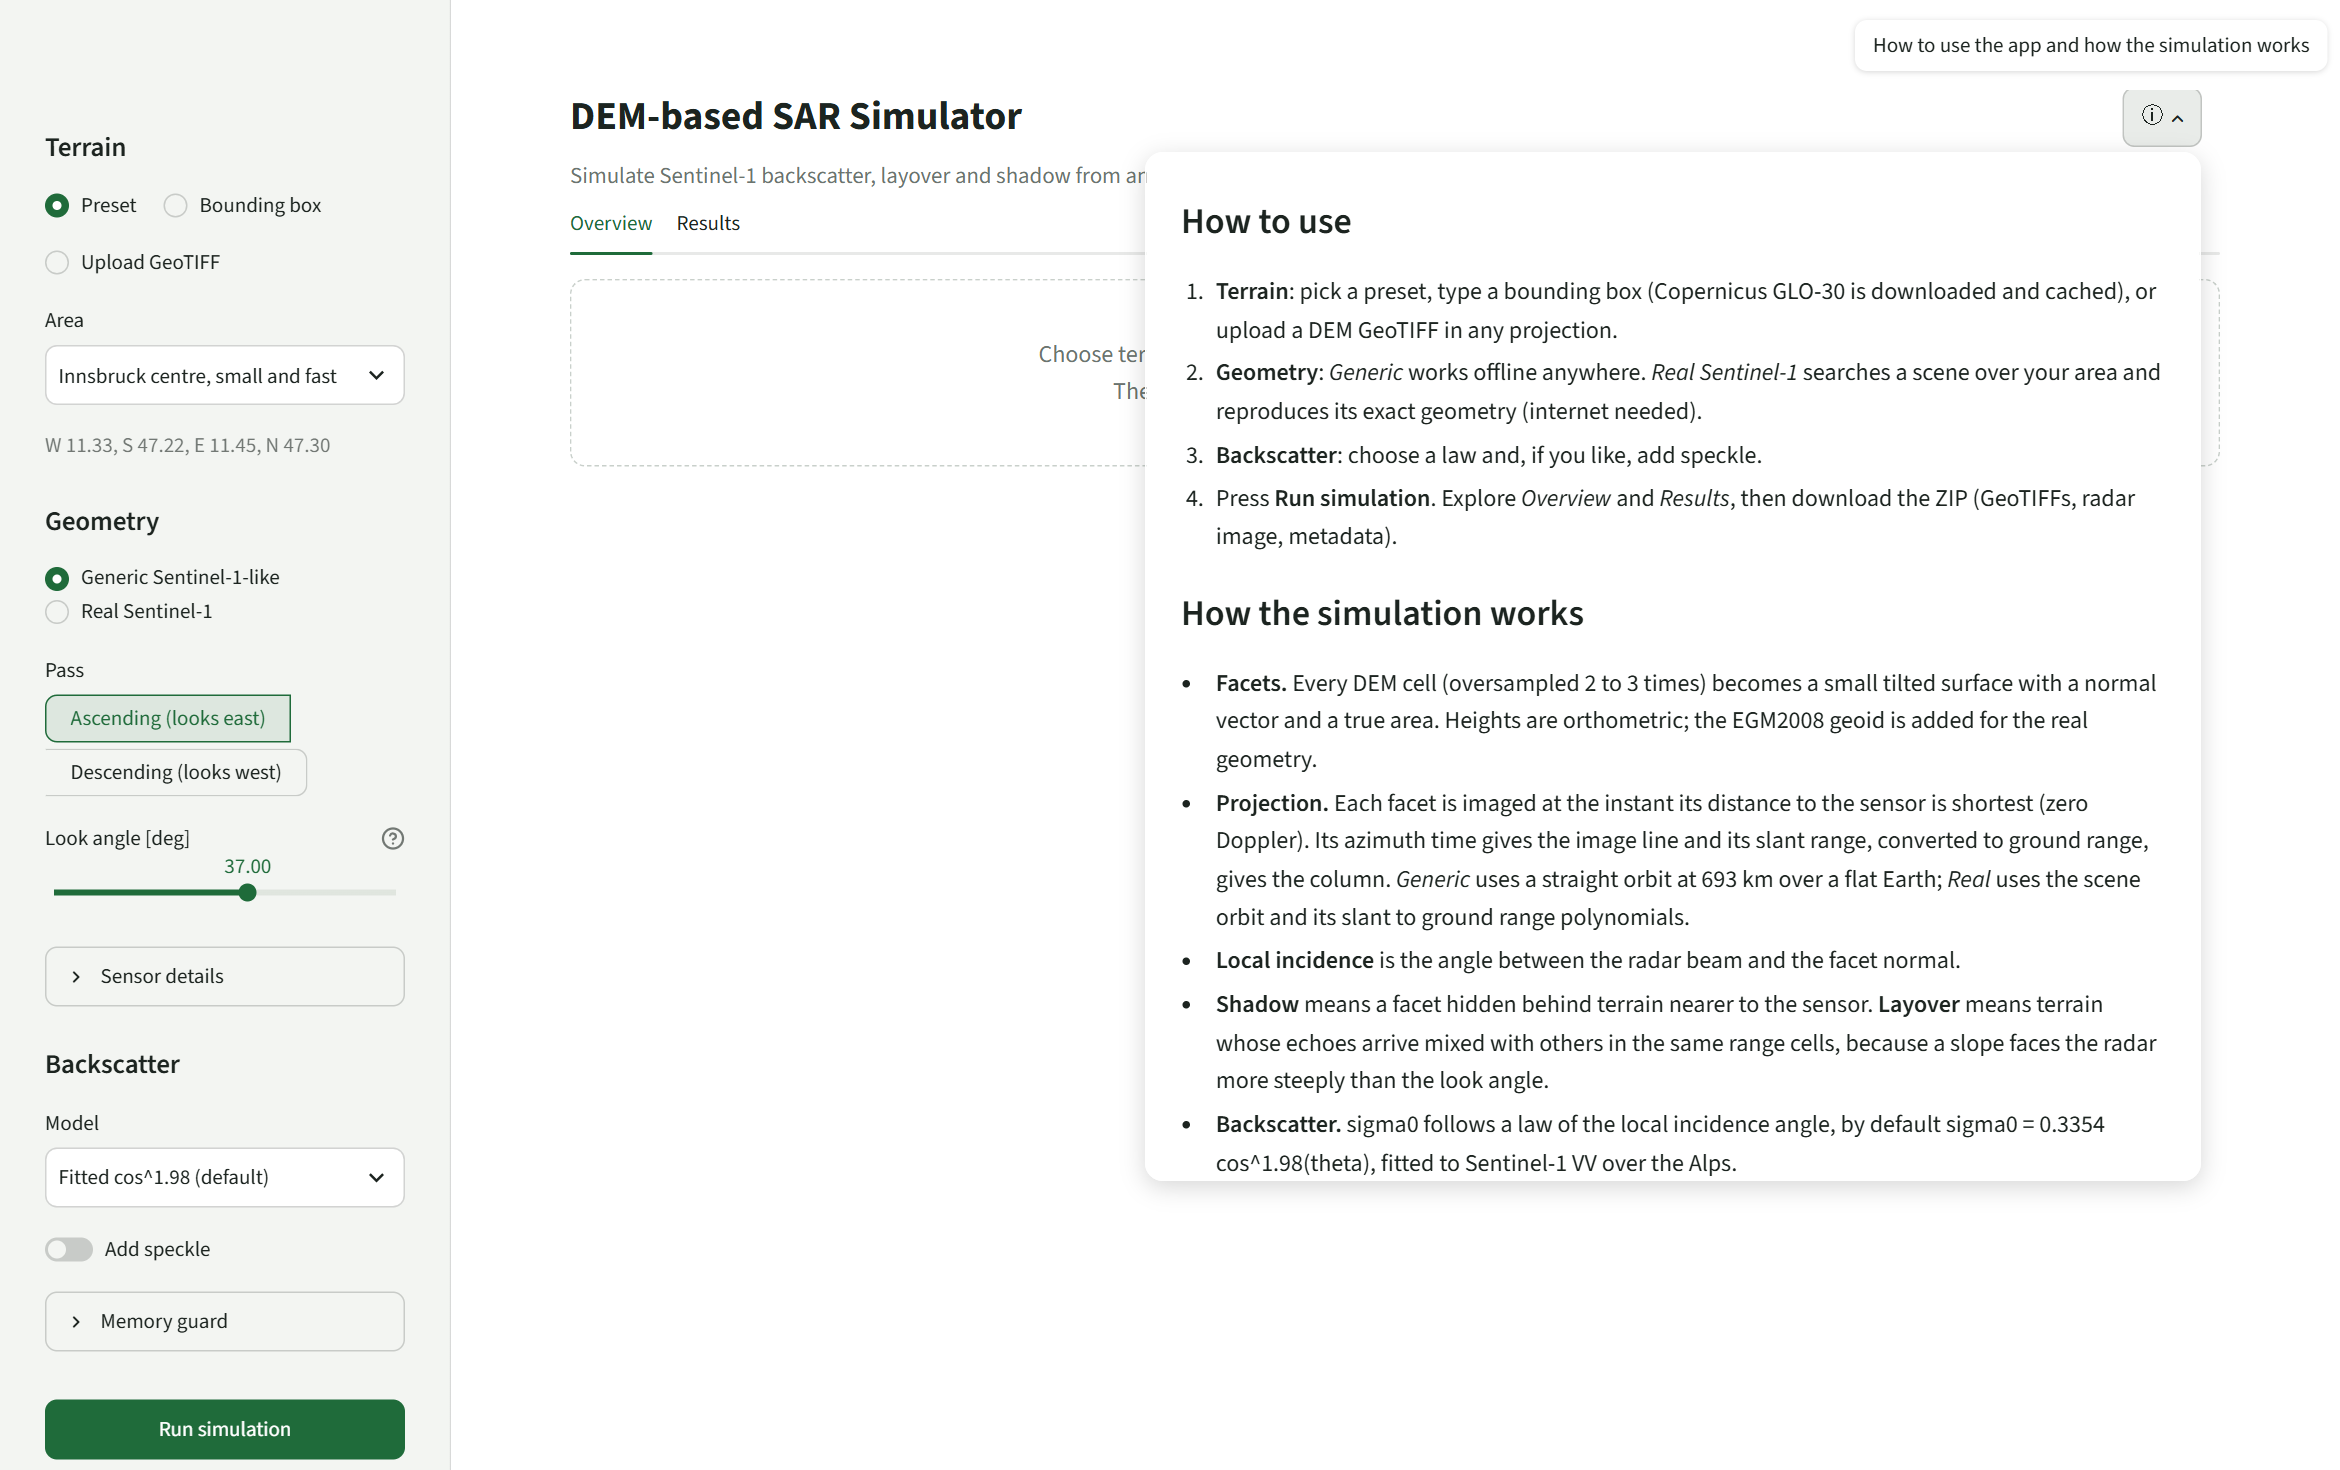
\includegraphics[width=\textwidth]{gui_02_info.png}
\caption[Graphical application: information panel]{Graphical application: information panel explaining how to use the
application and how the simulation works.}
\label{fig:gui-info}
\end{figure}
\begin{figure}[htbp]
\centering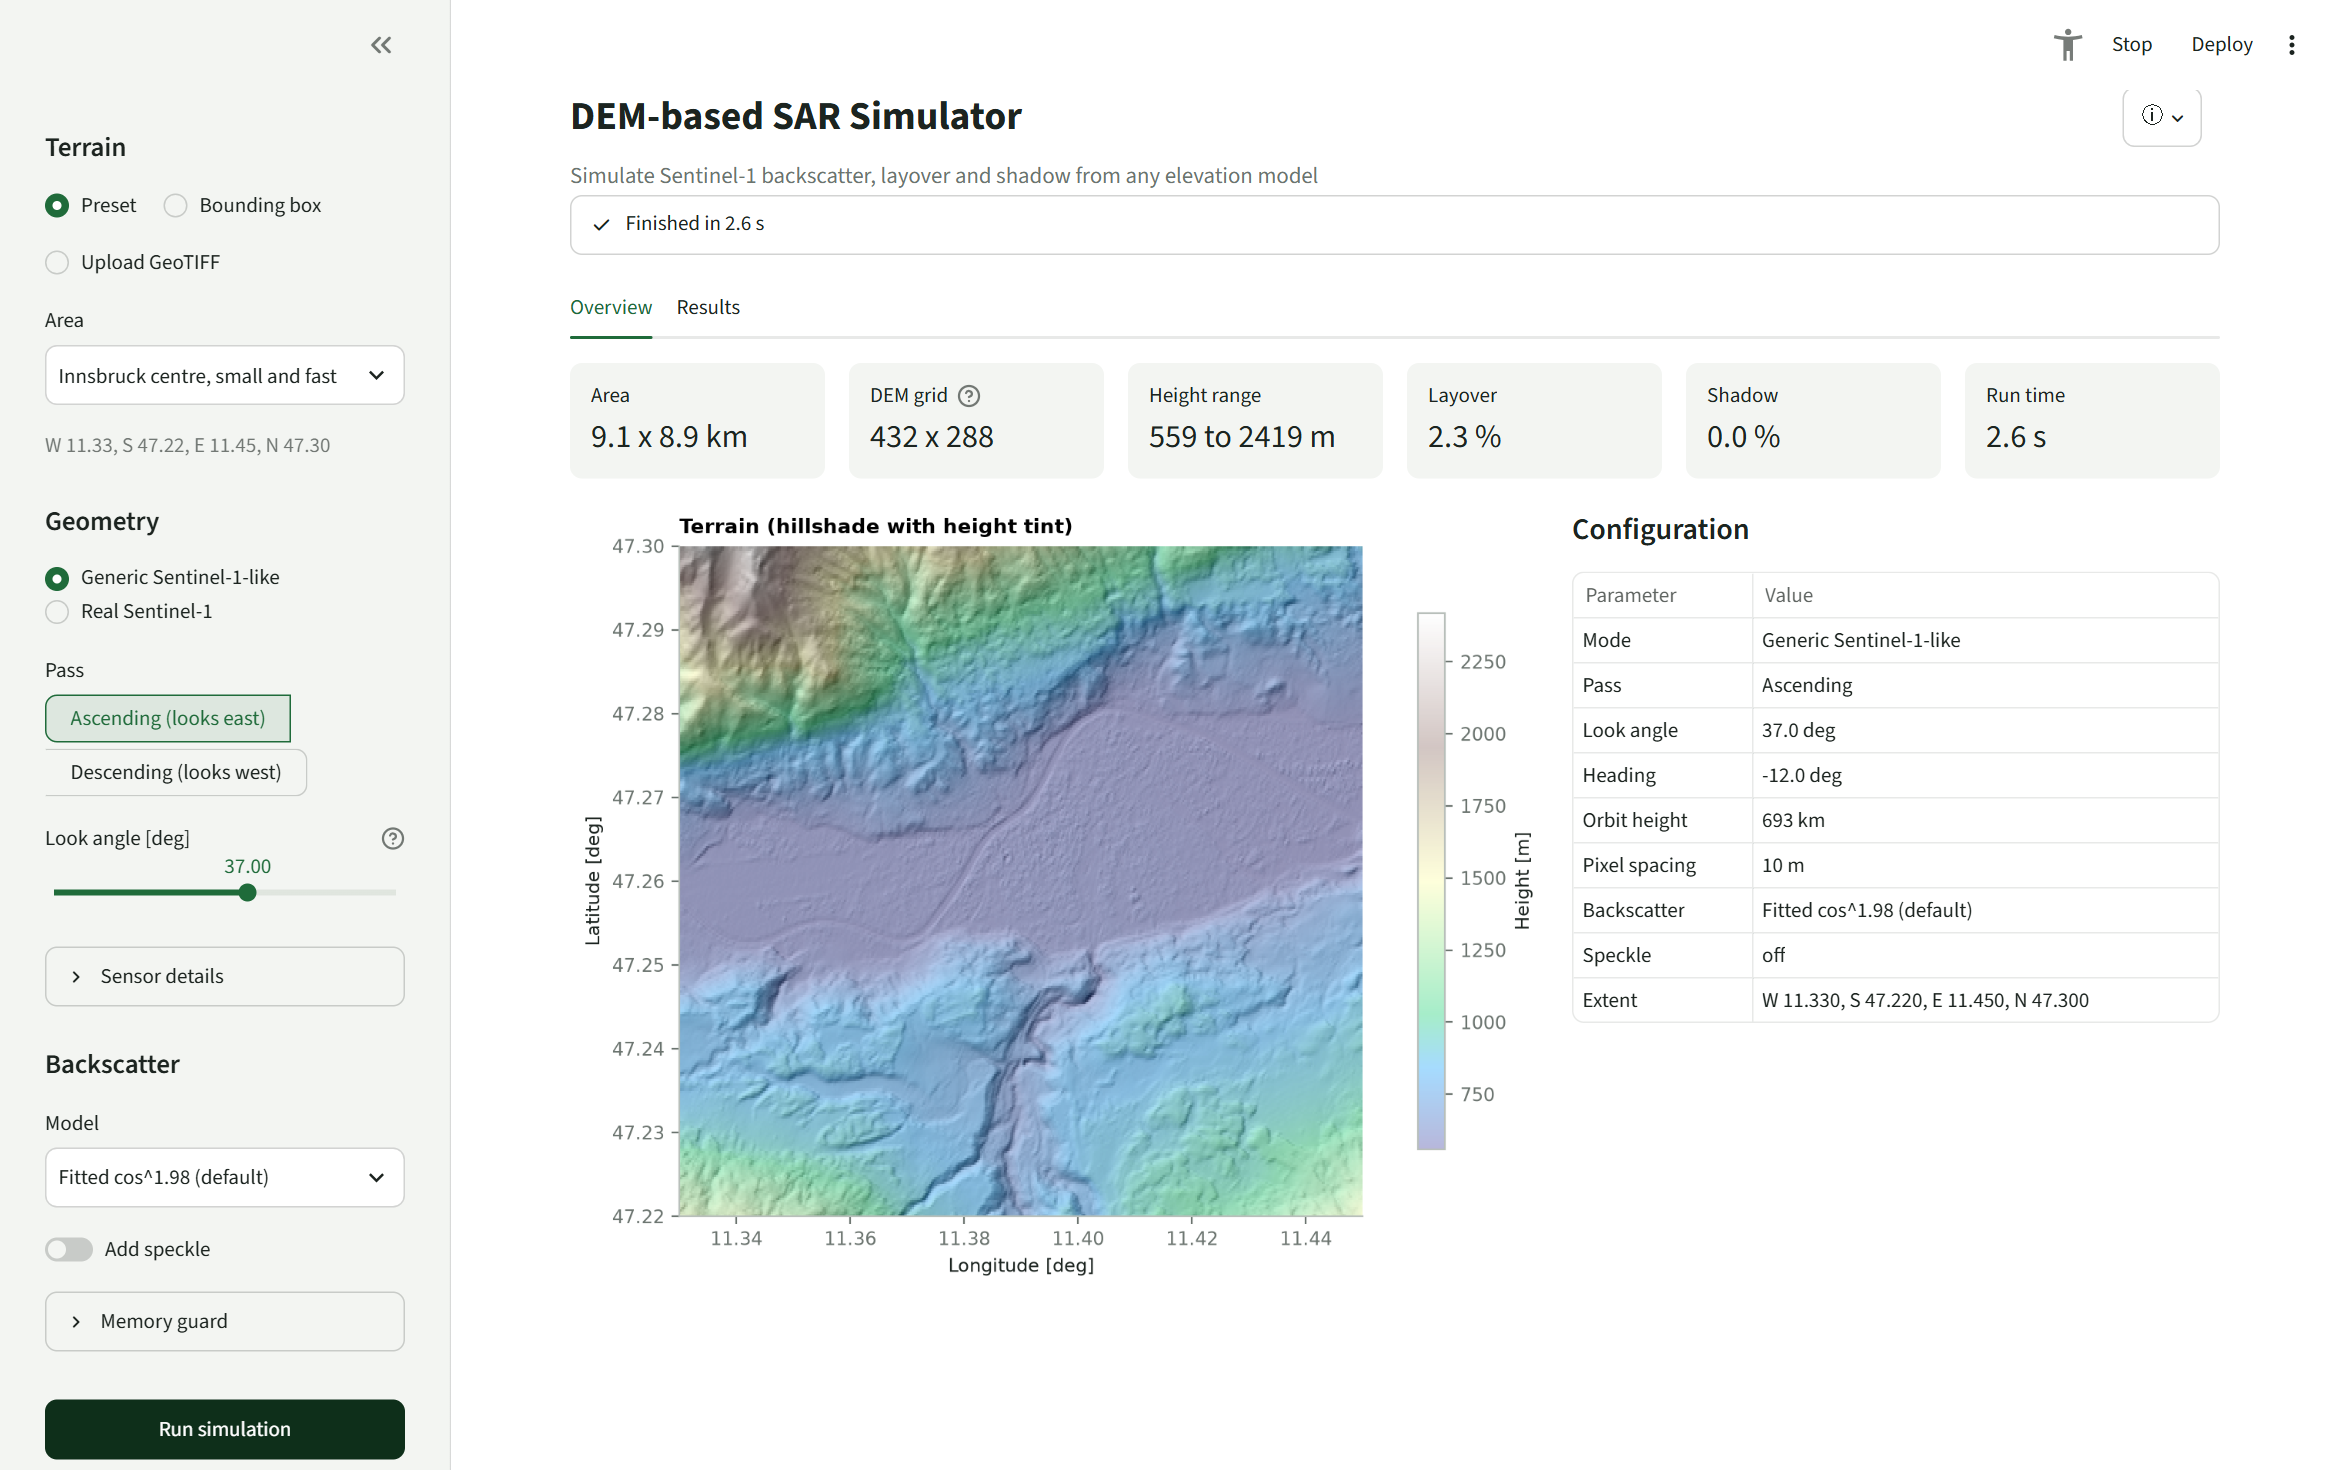
\includegraphics[width=\textwidth]{gui_03_overview.png}
\caption[Graphical application: Overview tab]{Graphical application: Overview tab after a run in the generic mode
over the Innsbruck preset, with summary cards, terrain hillshade and configuration.}
\label{fig:gui-overview}
\end{figure}
\begin{figure}[htbp]
\centering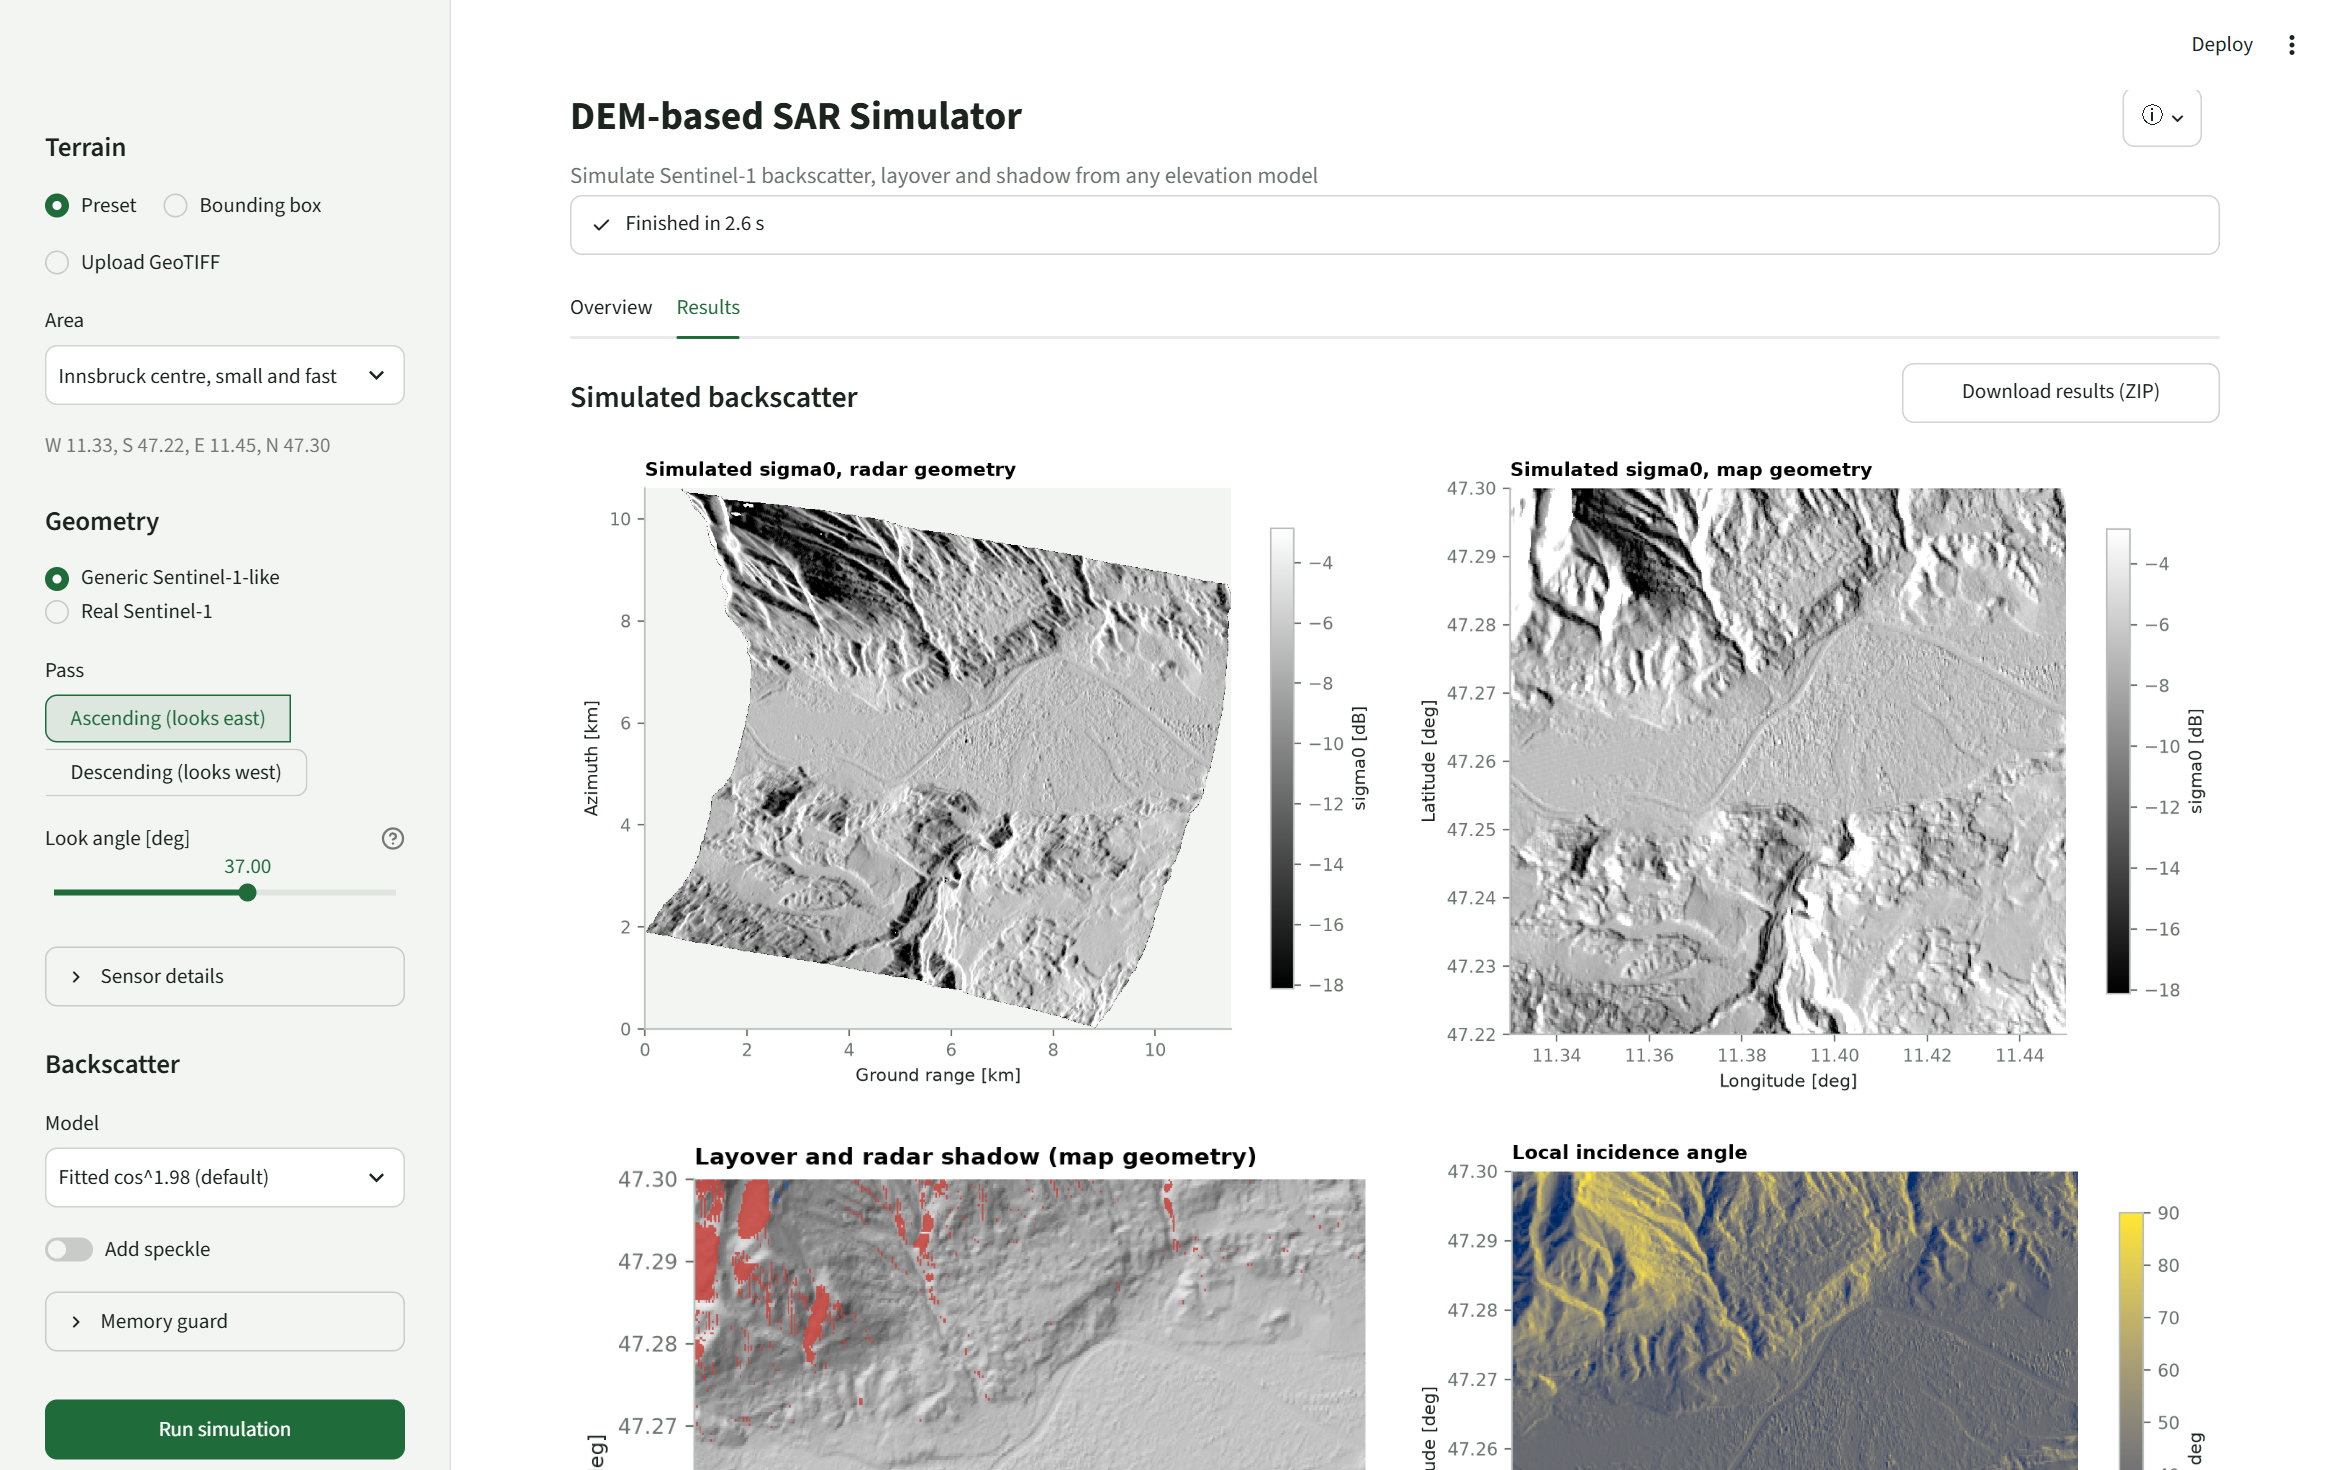
\includegraphics[width=\textwidth]{gui_04_results.png}
\caption[Graphical application: Results tab]{Graphical application: Results tab with the download button, the simulated
$\sigma^0$ in radar and map geometry, the layover and shadow masks and the local incidence angle.}
\label{fig:gui-results}
\end{figure}
